\documentclass[uplatex,dvipdfmx,a4paper,10pt]{jsarticle}
\usepackage{graphicx}
\usepackage{amsmath}
\usepackage{latexsym}
\usepackage{multirow}
\usepackage{url}
\usepackage[separate-uncertainty]{siunitx}
\usepackage{physics}
\usepackage{enumerate}
\usepackage{bm}
\usepackage{pdfpages}
\usepackage{pxchfon}
\usepackage{tikz}
\usepackage{float}
\usepackage{listings}

% lstlistingのsetting
\lstset{
    basicstyle={\ttfamily},
    identifierstyle={\small},
    commentstyle={\smallitshape},
    keywordstyle={\small\bfseries},
    ndkeywordstyle={\small},
    stringstyle={\small\ttfamily},
    frame={tb},
    breaklines=true,
    columns=[l]{fullflexible},
    numbers=left,
    xrightmargin=0zw,
    xleftmargin=3zw,
    numberstyle={\scriptsize},
    stepnumber=1,
    numbersep=1zw,
    lineskip=-0.5ex
}

% tikz setting
\usepackage{tikz}
\usetikzlibrary{automata, intersections, calc, arrows, positioning, arrows.meta}

% theories setting (for japanese language)
\usepackage{amsmath}
\usepackage{amsthm}

\theoremstyle{definition}
\newtheorem{thm}{定理}[section]
\newtheorem{lem}[thm]{補題}
\newtheorem{prop}[thm]{命題}
\newtheorem{cor}[thm]{系}
\newtheorem{ass}[thm]{仮定}
\newtheorem{conj}[thm]{予想}
\newtheorem{dfn}[thm]{定義}
\newtheorem{rem}[thm]{注}

\newtheorem*{thm*}{定理}
\newtheorem*{lem*}{補題}
\newtheorem*{prop*}{命題}
\newtheorem*{cor*}{系}
\newtheorem*{ass*}{仮定}
\newtheorem*{conj*}{予想}
\newtheorem*{dfn*}{定義}
\newtheorem*{rem*}{注}

% \renewcommand{\rmdefault}{pplj}
% \renewcommand{\sfdefault}{phv}

\setlength{\textwidth}{165mm} %165mm-marginparwidth
\setlength{\marginparwidth}{40mm}
\setlength{\textheight}{225mm}
\setlength{\topmargin}{-5mm}
\setlength{\oddsidemargin}{-3.5mm}
% \setlength{\parindent}{0pt}

\def\vector#1{\mbox{\boldmath $#1$}}
\newcommand{\AmSLaTeX}{%
 $\mathcal A$\lower.4ex\hbox{$\!\mathcal M\!$}$\mathcal S$-\LaTeX}
\newcommand{\PS}{{\scshape Post\-Script}}
\def\BibTeX{{\rmfamily B\kern-.05em{\scshape i\kern-.025em b}\kern-.08em
 T\kern-.1667em\lower.7ex\hbox{E}\kern-.125em X}}
\newcommand{\DeLta}{{\mit\Delta}}
\renewcommand{\d}{{\rm d}}
\def\wcaption#1{\caption[]{\parbox[t]{100mm}{#1}}}
\def\rm#1{\mathrm{#1}}
\def\tempC{^\circ \rm{C}}

\makeatletter
\def\section{\@startsection {section}{1}{\z@}{-3.5ex plus -1ex minus -.2ex}{2.3ex plus .2ex}{\Large\bf}}
\def\subsection{\@startsection {subsection}{2}{\z@}{-3.25ex plus -1ex minus -.2ex}{1.5ex plus .2ex}{\normalsize\bf}}
\def\subsubsection{\@startsection {subsubsection}{3}{\z@}{-3.25ex plus -1ex minus -.2ex}{1.5ex plus .2ex}{\small\bf}}
\makeatother

\makeatletter
\def\@seccntformat#1{\@ifundefined{#1@cntformat}%
   {\csname the#1\endcsname\quad}%      default
   {\csname #1@cntformat\endcsname}%    enable individual control
}

% proof enviroment
\renewenvironment{proof}[1][\proofname]{\par
  \pushQED{\qed}%
  \normalfont \topsep6\p@\@plus6\p@\relax
  \trivlist
  \item\relax
  {\bfseries
  #1\@addpunct{.}}\hspace\labelsep\ignorespaces
}{%
  \popQED\endtrivlist\@endpefalse
}
\makeatother

\newcommand{\tenexp}[2]{#1\times10^{#2}}


\begin{document}
% タイトル
\begin{center}
{\Large{\bf グラフとネットワーク 第12回宿題}} \\
{\bf 電気通信大学 Ⅰ類 コンピュータサイエンスプログラム 3年} \\
{\bf 2311081 木村慎之介} \\
\end{center}

\section{問2}
\hspace{1em}Petersenグラフの辺染色数が\(\chi'(G) = 4\)であることを証明する。
\begin{proof}[証明] \\
\hspace{1em}まず辺彩色については次の定理が成立する。

\begin{thm}
  任意のグラフ\(G\)に対し、\(\Delta(G) \leq \chi'(G) \leq \Delta(G) + 1\)が成立する。
\end{thm}

Petersonグラフは\(3\)正則グラフであるから\(\Delta(G) = 3\)であるため、Petersonグラフは多くとも\(4\)色で辺彩色することができる。
よって、\(\chi'(G) = 4\)であることを示すには\(3\)色ではPetersonグラフを辺彩色することができないことを示せばいい。
以降、Petersonグラフが\(3\)色で辺彩色可能であると仮定して、その矛盾を導くことで証明する。

Petersonグラフが\(3\)色で辺彩色であることを仮定する。
さて、Petersonグラフは以下のグラフと同型である。

\begin{figure}[H]
  \centering
  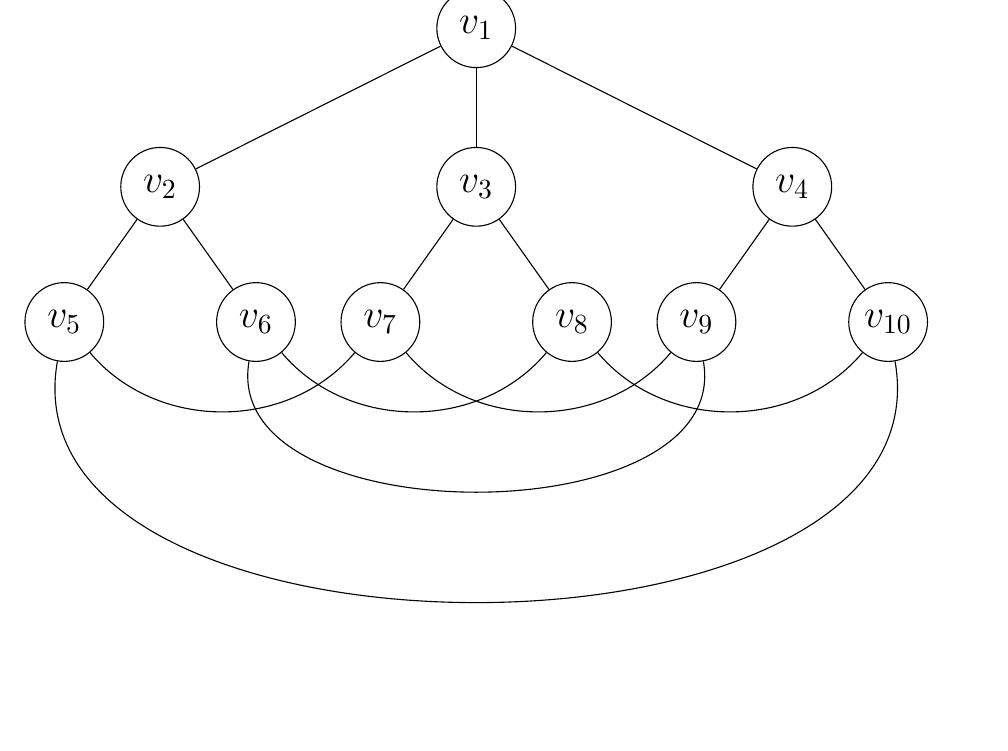
\begin{tikzpicture}[every node/.style={circle, draw, font=\Large, minimum size=1cm}]
    % setting node
    \node (v_1) {\(v_1\)};
    \node[below=1cm of v_1] (v_3) {\(v_3\)};
    \node[left=3cm of v_3] (v_2) {\(v_2\)};
    \node[right=3cm of v_3] (v_4) {\(v_4\)};
    \node[below left = 1cm and 0.5cm of v_2] (v_5) {\(v_5\)};
    \node[below right = 1cm and 0.5cm of v_2] (v_6) {\(v_6\)};
    \node[below left = 1cm and 0.5cm of v_3] (v_7) {\(v_7\)};
    \node[below right = 1cm and 0.5cm of v_3] (v_8) {\(v_8\)};
    \node[below left = 1cm and 0.5cm of v_4] (v_9) {\(v_9\)};
    \node[below right = 1cm and 0.5cm of v_4] (v_10) {\(v_{10}\)};

    % setting path
    \draw (v_1) -- (v_2);
    \draw (v_1) -- (v_3);
    \draw (v_1) -- (v_4);

    \draw (v_2) -- (v_5);
    \draw (v_2) -- (v_6);

    \draw (v_3) -- (v_7);
    \draw (v_3) -- (v_8);

    \draw (v_4) -- (v_9);
    \draw (v_4) -- (v_10);

    \draw[bend right=50] (v_5) to (v_7);
    \draw[bend right=50] (v_7) to (v_9);
    \draw[bend left=100] (v_9) to (v_6);
    \draw[bend right=50] (v_6) to (v_8);
    \draw[bend right=50] (v_8) to (v_10);
    \draw[bend left=100] (v_10) to (v_5);
  \end{tikzpicture}
\end{figure}

さて、仮定よりこのグラフは\(3\)辺彩色可能なので\(\{v_1, v_2\}\)に赤色、\(\{v_1, v_3\}\)に青色、\(\{v_1, v_4\}\)に緑色を割り当てる。
なお、このように辺の色を固定して考えてもグラフの対称性から一般性を失うことはない。
ここで、\(\{v_5, v_{10}\}\)について次の3つのパターンを考える。

\begin{enumerate}
  \item \(\{v_5, v_{10}\}\)の色が青色の時
  \item \(\{v_5, v_{10}\}\)の色が赤色の時
  \item \(\{v_5, v_{10}\}\)の色が青色の時
\end{enumerate}

\noindent Petersenグラフが3彩色可能という仮定から、このグラフは\(\{v_5, v_{10}\}\)が赤、青、緑のいずれかの色の時に3彩色できる割当パターンを持つため、この3つについて調べれば良い。
なお、2と3については対称性から彩色可能か否かの結果が一致するため今回は1と2のみを調べる。 \\

ここで、彩色のやり方について次の2つのパターンに当てはめながら彩色を行っていく。

\begin{itemize}
  \item 頂点\(v_i\)について、この頂点から伸びている2つの辺の色が決定している場合は、残りの色を彩色されていない辺に割り当てる。
  \item 辺\(\{v_i, v_j\}\)について、\(v_i\)と\(v_j\)それぞれについて\(\{v_i, v_i\}\)以外の端点となる辺の色が彩色されており、それぞれで彩色された色が異なる場合に、残りの色を\(\{v_i, v_j\}\)に割り当てる。
\end{itemize}

\(\{v_5, v_{10}\}\)が青色の時、Petersenグラフが3彩色可能であることから、次のように辺に割り当てる色が決定していく。

\begin{enumerate}
  \item \(\{v_{10}, v_4\}\)に赤を割り当てる
  \item \(\{v_{10}, v_8\}\)に緑を割り当てる
  \item \(\{v_8, v_3\}\)に赤を割り当てる
  \item \(\{v_3, v_7\}\)に緑を割り当てる
  \item \(\{v_7, v_9\}\)に青を割り当てる
  \item \(\{v_9, v_4\}\)に赤を割り当てる
\end{enumerate}

しかし、このように色を割り当てていくと\(v_4\)を端点とする2つの辺\(\{v_4, v_9\}\)と\(\{v_4, v_{10}\}\)が赤色となり彩色可能なことに矛盾する。

一方\(\{v_5, v_{10}\}\)が赤色の時、Petersenグラフの彩色は以下のように決定していく。

\begin{enumerate}
  \item \(\{v_{10}, v_4\}\)に青を割り当てる
  \item \(\{v_{10}, v_8\}\)に緑を割り当てる
  \item \(\{v_8, v_3\}\)に赤を割り当てる
  \item \(\{v_8, v_6\}\)に青を割り当てる
  \item \(\{v_6, v_2\}\)に緑を割り当てる
  \item \(\{v_2, v_5\}\)に青を割り当てる
  \item \(\{v_5, v_7\}\)に緑を割り当てる
\end{enumerate}

しかし、このように色を割り当てていくと\(v_7\)を端点とする2つの辺\(\{v_7, v_5\}\)と\(\{v_7, v_3\}\)が緑色となり彩色可能なことに矛盾する。

以上よりいずれの場合においても彩色可能であることに矛盾することがわかったため、Petersenグラフは3彩色可能なグラフではないことがわかる。
故にPetersenのグラフを彩色するのに必要な色の最小の数は\(4\)つとなる。
\end{proof}


%%%%%%%%%%%%%%%%%%%%%%%%%%%%%%%%%%%%%%%%%%%%%%%%%%%%%%%%%%%%%%%%%%%%%%
\appendix
\setcounter{figure}{0}
\setcounter{table}{0}
\numberwithin{equation}{section}
\renewcommand{\thetable}{\Alph{section}\arabic{table}}
\renewcommand{\thefigure}{\Alph{section}\arabic{figure}}
%\def\thesection{付録\Alph{section}}
\makeatletter 
\newcommand{\section@cntformat}{付録 \thesection:\ }
\makeatother
%%%%%%%%%%%%%%%%%%%%%%%%%%%%%%%%%%%%%%%%%%%%%%%%%%%%%%%%%%%%%%%%%%%%%%

    
\end{document}